\documentclass[12pt]{beamer}
\usepackage{amsmath}
\usepackage{mathtools}
\usepackage{multimedia}
\usepackage{hyperref}


\usefonttheme{professionalfonts} % using non standard fonts for beamer
\usefonttheme{serif} % default family is serif
%\documentclass[12pt]{beamerthemeSam.sty}
\usepackage{epsf}
%\usepackage{pstricks}
%\usepackage[orientation=portrait,size=A4]{beamerposter}
\geometry{paperwidth=160mm,paperheight=120mm}
%DT favorite definitions
\def\LL{\left\langle}	% left angle bracket
\def\RR{\right\rangle}	% right angle bracket
\def\LP{\left(}		% left parenthesis
\def\RP{\right)}	% right parenthesis
\def\LB{\left\{}	% left curly bracket
\def\RB{\right\}}	% right curly bracket
\def\PAR#1#2{ {{\partial #1}\over{\partial #2}} }
\def\PARTWO#1#2{ {{\partial^2 #1}\over{\partial #2}^2} }
\def\PARTWOMIX#1#2#3{ {{\partial^2 #1}\over{\partial #2 \partial #3}} }

\def\rightpartial{{\overrightarrow\partial}}
\def\leftpartial{{\overleftarrow\partial}}
\def\diffpartial{\buildrel\leftrightarrow\over\partial}

\def\BCC{\begin{columns}}
\def\ECC{\end{columns}}
\def\HC{\column{0.5\textwidth}}
\def\BC{\begin{center}}
\def\EC{\end{center}}
\def\BN{\begin{enumerate}}
\def\EN{\end{enumerate}}
\def\BI{\begin{itemize}}
\def\EI{\end{itemize}}
\def\BE{\begin{displaymath}}
\def\EE{\end{displaymath}}
\def\BEA{\begin{eqnarray*}}
\def\EEA{\end{eqnarray*}}
\def\BNEA{\begin{eqnarray}}
\def\ENEA{\end{eqnarray}}
\def\EL{\nonumber\\}

\newcommand{\etal}{{\it et al.}}
\newcommand{\gbeta}{6/g^2}
\newcommand{\la}[1]{\label{#1}}
\newcommand{\ie}{{\em i.e.\ }}
\newcommand{\eg}{{\em e.\,g.\ }}
\newcommand{\cf}{cf.\ }
\newcommand{\BS}{\bigskip}
\newcommand{\etc}{etc.\ }
\newcommand{\atantwo}{{\rm atan2}}
\newcommand{\Tr}{{\rm Tr}}
\newcommand{\dt}{\Delta t}
\newcommand{\op}{{\cal O}}
\newcommand{\msbar}{{\overline{\rm MS}}}
\def\chpt{\raise0.4ex\hbox{$\chi$}PT}
\def\schpt{S\raise0.4ex\hbox{$\chi$}PT}
\def\MeV{{\rm Me\!V}}
\def\GeV{{\rm Ge\!V}}

%AB: my color definitions
%\definecolor{mygarnet}{rgb}{0.445,0.184,0.215}
%\definecolor{mygold}{rgb}{0.848,0.848,0.098}
%\definecolor{myg2g}{rgb}{0.647,0.316,0.157}
\definecolor{A}{rgb}{1.0,0.3,0.3}
\definecolor{B}{rgb}{0.0,1.0,0.0}
\definecolor{C}{rgb}{1.0,1.0,0.0}
\definecolor{D}{rgb}{0.5,0.5,1.0}
\definecolor{E}{rgb}{0.7,0.7,0.7}
\definecolor{abtitlecolor}{rgb}{1.0,1.0,1.0}
\definecolor{absecondarycolor}{rgb}{0.0,0.416,0.804}
\definecolor{abprimarycolor}{rgb}{1.0,0.686,0.0}
\definecolor{Red}           {rgb}{1,0.4,0.4}
\definecolor{Yellow}           {rgb}{1,1,0.0}
\definecolor{Grey}          {cmyk}{.7,.7,.7,0}
\definecolor{Blue}          {cmyk}{1,1,0,0}
\definecolor{Green}         {cmyk}{1,0,1,0}
\definecolor{Brown}         {cmyk}{0,0.81,1,0.60}
\definecolor{Silver}        {rgb}{0.95,0.9,1.0}
\definecolor{Sky}           {rgb}{0.07,0.0,0.2}
\definecolor{Darkbrown}     {rgb}{0.4,0.3,0.2}
\definecolor{Black}         {rgb}{0.0,0.0,0.0}
\definecolor{40Gray}        {rgb}{0.4,0.4,0.5}
\usetheme{Madrid}


\setbeamercolor{normal text}{fg=Silver,bg=Sky}

%AB: redefinition of beamer colors
%\setbeamercolor{palette tertiary}{fg=white,bg=mygarnet}
%\setbeamercolor{palette secondary}{fg=white,bg=myg2g}
%\setbeamercolor{palette primary}{fg=black,bg=mygold}
\setbeamercolor{title}{fg=abtitlecolor}
\setbeamercolor{frametitle}{fg=abtitlecolor}
\setbeamercolor{palette tertiary}{fg=white,bg=Darkbrown}
\setbeamercolor{palette secondary}{fg=white,bg=absecondarycolor}
\setbeamercolor{palette primary}{fg=white,bg=40Gray}
\setbeamercolor{structure}{fg=abtitlecolor}

\setbeamerfont{section in toc}{series=\bfseries}

%AB: remove navigation icons
\beamertemplatenavigationsymbolsempty
\title[Light and matter]{
  \textbf {Light and matter}}

\author [Astronomy 101]{Astronomy 101\\Syracuse University, Fall 2021\\Walter Freeman}

\date{\today}

\begin{document}



\frame{\titlepage}

\frame{
\BC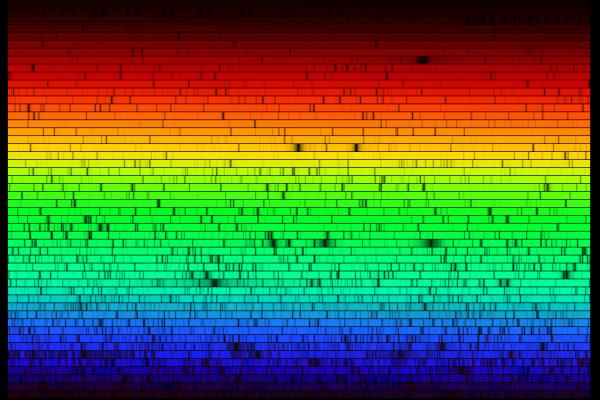
\includegraphics[width=\textwidth]{solarspectrum.jpg}\EC
}

\frame{\frametitle{\textbf{Announcements}}
\large
\BI
\item Your paper is due Thursday, November 3.  If you need an extension, please let us know in advance and tell us why.
\item If you have questions about your paper, come to office hours or ask in {\tt \#paper-questions} on Discord.
\pause
\bigskip
\item If you are looking for extra help with your paper, bring a draft to office hours or send it to Kiersten Edwards, our writing coach, at {\tt kedwar03@syr.edu} or on Discord.
\EI
\pause\BS\BS\BS
\color{B} \BC Are there any questions about the paper? \EC
}


\frame{\frametitle{\textbf{Announcements}}
	\BC
	\color{A} \Large
	``I can't think of a good topic!''
	\EC
	
	\BI
	\item We want you to pick a topic that {\it you} care about.
	\item You don't have to pick from our examples!
	\item Be careful of ``defaults'' (Stanford prison experiment) made famous elsewhere
	\EI
	\BS\BS
	
	\pause
	\color{B}
	The best topics are:
	\BI
	\item Topics that are relevant to today's society
	\item Things {\it you} care about
	\item Not necessarily ``scientific journal articles'' (science is more broad than that!)
	\EI
	
	\pause\BS\BS
	
	\color{C}Example: My conversation with someone yesterday about basketball...
}


\frame{\frametitle{\textbf{Announcements}}
	\Large
	
	\BC
	The physics building is not in fact on fire, but there was a fire alarm this morning!
	\EC
	
}

\frame{\frametitle{\textbf{Last time}}
\Large
\BC
Last time we saw that all objects with a temperature emit a broad spectrum of light.
\EC

As an object gets hotter, the light coming from it:

\BI
\item ... becomes brighter
\item ... shifts to shorter wavelengths (``becomes bluer'')
\EI
}


\frame{
	
	\huge
	
	\BC
	Let's practice this.
	

	\EC
}

\frame{

\BC
\Large
Which of these stars is hottest?

\BS

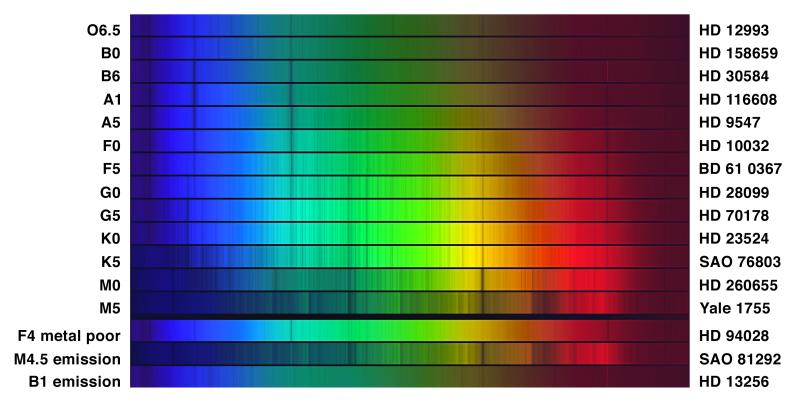
\includegraphics[width=0.95\textwidth]{stellar-spectra.jpg}
\BS
\EC
\huge
\BCC
\HC
\color{A}A: O6.5 \\
\color{C}C: G5
\HC
\color{B}B: K5 \\
\color{D}D: F4 ``metal poor''
\ECC
}


\frame{\frametitle{\textbf{Chemistry done ${\rm \bf quick}^{\dagger}$}}

\BC
\large
Electrons in an atom can only have {\bf particular} amounts of energy!

\BS

We call these ``energy levels'', and measure their energy in ``electron volts'' (eV).

\EC

\BI
\item Usually all the electrons live in the lowest available levels
\item There's a limit to how many electrons can be in each level
\item Atoms ``fill up'' the levels starting from the bottom
\item This process leads to the periodic table
\EI
\pause
\begin{flushright}\scriptsize $\dagger$ Does not replace your introductory chemistry class on your transcript\end{flushright}
}

\frame{\frametitle{\textbf{Atomic transitions}}
	\Large
	
	Each electron lives in one of these energy levels at all times. 
	
	\BS
	
	They are not physical locations, but patterns of orbiting the nucleus. Higher energy levels orbit further away.
	
	\BS
	
	They {\bf cannot} be in between.
	
	\BS
	
	If you add energy, you can move an electron to a higher energy level.
}


\frame{\frametitle{\textbf{Atomic transitions}}

\Large

Here's a sample atom (on the document camera). These numbers aren't real; I just made them up for demonstration.

\BS

Can the electron in this atom go from $n=1$ (``ground state'') to $n=2$ (an ``excited state'')?

\BS

\color{A}A: Yes, since it's just moving from here to there \\ \BS
\color{B}B: Yes, but only if I give it 4 eV of energy from somewhere \\ \BS
\color{C}C: No, because atoms have a definite state \\ \BS
\color{D}D: No, because that doesn't conserve energy
}


\frame{\frametitle{\textbf{Atomic transitions: absorption}}

\large

This extra energy usually comes from a {\it photon} -- a particle of light.

Remember that photons carry energy with them: the shorter the wavelength,
the higher the energy.

\BC
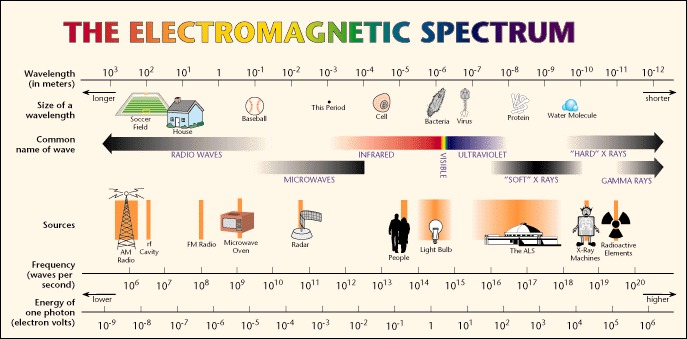
\includegraphics[width=0.8\textwidth]{EMSpec.jpg}
\EC

\large

An atom can absorb a photon with
just the right energy,  jumping
up to a higher energy level in the process.
}

\frame{
\Large
What energies of photon can our sample atom absorb if it starts in $n=1$?

\BS\BS
\Large
\color{A}A: 4 eV\\ \BS
\color{B}B: 4 eV, 3 eV, 2 eV, or 1 eV\\ \BS
\color{C}C: 4 eV, 7 eV, 9 eV, or 10 eV\\ \BS
\color{D}D: Any value up to 10 eV \\ \BS
\color{E}E: Any value between 4 eV and 10 eV \\
}

\frame{
	\Large
	What energies of photon can our sample atom absorb if it starts in $n=2$?
	
	\BS\BS
	\Large
	\color{A}A: 3 eV\\ \BS
	\color{B}B: 4 eV, 3 eV, 2 eV, or 1 eV\\ \BS
	\color{C}C: 3 eV, 5 eV, or 6 eV\\ \BS
	\color{D}D: 4 eV \\ \BS
	\color{E}E: Any value between 3 eV and 6 eV \\
}


\frame{
\Large

If an atom is in an excited state (maybe because it has absorbed a photon), it can
transition downward, spitting out photons in the process.

\BS

It may make {\bf any} allowed transition that jumps between energy levels.

\BS
}

\frame{
	
	\Large
Suppose our atom starts in the $n=3$ energy level. What could it do?	


	\BS\BS
	\Large
	\color{A}A: Emit a 3 eV photon\\ \BS
	\color{B}B: Absorb a 3 eV photon\\ \BS
	\color{C}C: Emit a 7 eV photon\\ \BS
	\color{D}D: Absorb a 2 eV photon\\ \BS
	\color{E}E: Emit a 4 eV photon
}


\frame{
\Large
Suppose our atom absorbs a photon of 9 eV. What happens?

\BS\BS
\Large
\color{A}A: It will emit a photon of 9 eV \\ \BS 
\color{B}B: It will emit a 2 eV photon, then a 7 eV photon\\ \BS
\color{C}C: It will emit a 5 eV photon, then a 4 eV photon\\ \BS
\color{D}D: It will emit a 2 eV photon, then a 3 eV photon, then a 4 eV photon\\ \BS
\color{E}E: It will emit a 3 eV photon, then a 6 eV photon\\
}



\frame{\frametitle{\bf Chemistry: all I want you to know}
\large
\BI
\item Electrons occupy certain {\bf energy levels}
\item The particular energies that these levels have is {\bf unique} to particular elements: hydrogen has different allowed energies than mercury or neon or sodium etc.
\item An atom can absorb a photon and jump up to a higher level, conserving energy
\item ... an atom in a higher level can emit photons, jumping back down, conserving energy.
\item {\color{Red}``Nature does not make change''}
\EI

\BS
\BS
\BC ... that's it. :) 
\EC
}

\frame{

If I take hydrogen and tear the electrons off of the atoms with an electric current,
they'll ``fall'' back down, going through the energy levels down to $n=1$.

\BS

Sometimes they'll skip energy levels; sometimes they'll go in sequence.

\BS

Suppose a hydrogen atom is in the $n=4$ state. What color and energy will it emit if it jumps to $n=3$? 

\BS\BS

\color{A}A: 0.7 eV (Red) \\
\color{B}B: 12.8 eV (Ultraviolet) \\
\color{C}C: 0.7 eV (Infrared)  \\
\color{D}D: 2.3 eV (Cyan) \\
\color{E}E: None of the above

}

\frame{
	
	If I take hydrogen and tear the electrons off of the atoms with an electric current,
	they'll ``fall'' back down, going through the energy levels down to $n=1$.
	
	\BS
	
	Sometimes they'll skip energy levels; sometimes they'll go in sequence.
	
	\BS
	
	Suppose a hydrogen atom is in the $n=4$ state. What color and energy will it emit if it jumps to $n=2$? 
	
	\BS\BS
	
\color{A}A: 10.2 eV (Ultraviolet) \\
\color{B}B: 12.8 eV (Ultraviolet) \\
\color{C}C: 0.4 eV (Infrared) \\
\color{D}D: 2.6 eV (Cyan) \\
\color{E}E: None of the above
}



\frame{

If I do this to hydrogen, what color will it produce? (For reference: the visible range is 1.6-3.2 eV.)

\BS
\BS

\color{A}A: UV: we won't see it, since the transitions down to $n=1$ are in the UV\\

\BS

\color{B}B: Several colors of visible light: we'll see the transitions down to $n=2$, which are visible\\ 

\BS

\color{C}C: Infrared: the transitions at the top are very low energy, corresponding to
infrared light which we can't see \\ 

\BS

\color{D}D: UV, IR, and visible, all at once: all the transitions happen, but we only see the
visible photons because of the limits of our eyes\\ 

\BS

\pause

\color{E}E: Orange, because this is Syracuse, darnit! 
}

%\frame{
%\Large
%\BC
%Complete {\it Lecture Tutorials} pp.65-69.
%
%\BS
%\BS
%\normalsize
%After this, we'll talk about another application of this idea.
%\EC}

\frame{\frametitle{\bf Emission spectra}

\large

Every chemical element has a unique {\it spectrum}: the colors of light that it can emit and absorb.

\BS

Other colors simply pass through.

\BS

(Molecules have these spectra too: their electron energy levels are more complicated.)
}



\frame{
	
	\BC
	\Large
	Suppose I put a 5000 K object behind a cloud of gas with energy levels at 0, 3, and 5 eV. What does the 5000 K object do?
	\EC
	\BS
	\BS
	
	\Large
	\color{A}A: Emit light of a broad range of wavelengths \\
	
	\BS
	
	\color{B}B: Absorb light of a broad range of wavelengths \\
	
	\BS
	
	\color{C}C: Emit light made of 3 and 5 eV photons \\
	
	
	\BS
	
	\color{D}D: Absorb light made of 3 and 5 eV photons \\
	
	\BS
}


\frame{
	
	\BC
	\Large
	Suppose I put a 5000 K object behind a cloud of gas with energy levels at 0, 3, and 5 eV. What could this cloud of gas do?
	\EC
	\BS
	\BS
	
	\Large
	\color{A}A: Emit light of a broad range of wavelengths  \\
	
	\BS
	
	\color{B}B: Absorb light of a broad range of wavelengths \\
	
	\BS
	
	\color{C}C: Absorb photons with at least 2 eV of energy \\
	
	
	\BS
	
	\color{D}D: Absorb photons of 2, 3 and 5 eV, and allow the rest to pass \\
	
	\BS
}


\frame{

\BC
\Large
Suppose I put a 5000 K object behind a cloud of gas with energy levels at 0, 3, and 5 eV, and then look at the 
energies of the photons that come out the other side. 
\EC
\BS
\BS

\Large
\color{A}A: Photons with energy 3 and 5 eV \\

\BS

\color{B}B: Photons with energy 2, 3, and 5 eV \\

\BS

\color{C}C: Photons of a wide range of energies, {\it except} 3 and 5 eV \\


\BS

\color{D}D: Photons of a wide range of energies, {\it except} 2, 3, and 5 eV \\

\BS
}

\frame{

\BC
\Large
Suppose I put a 5000 K object behind a cloud of gas with energy levels at 0, 3, and 5 eV, and then 
separate its light by color. (Assume that I am a bird and can see ultraviolet light.) What would I see?
\EC
\BS
\BS

\Large
\color{A}A: Only two bright lines \\ 

\BS

\color{B}B: Only three bright lines \\ 

\BS

\color{C}C: A solid band of color, but with two dark lines \\ 


\BS

\color{D}D: A solid band of color, but with three dark lines \\ 

\BS

}


\frame{

\BC
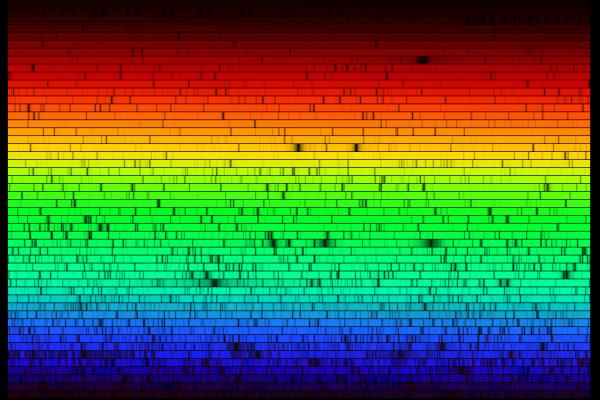
\includegraphics[width=0.7\textwidth]{solarspectrum.jpg}
\EC

\BI
\item The hot core of the Sun emits light of all wavelengths (thermal radiation)
\pause
\item The gases in the cooler atmosphere absorb light of their particular wavelengths
\pause
\EI
\BC
\color{Red} \large This picture tells us what's in the Sun!
\EC
}

\frame{

\Large

You discover lines in the solar spectrum that don't correspond to any known element.
What do you conclude?

\BS

\color{A}A: Something about quantum mechanics is different in the Sun\\\BS

\color{B}B: Something about light is different in the Sun\\\BS
\color{C}C: There's an element in the Sun that's not on Earth -- call it {\bf sunium} \\ \BS
\color{D}D: The extreme temperature of the Sun causes new lines to appear in its gas \\
}


\frame{

\BC
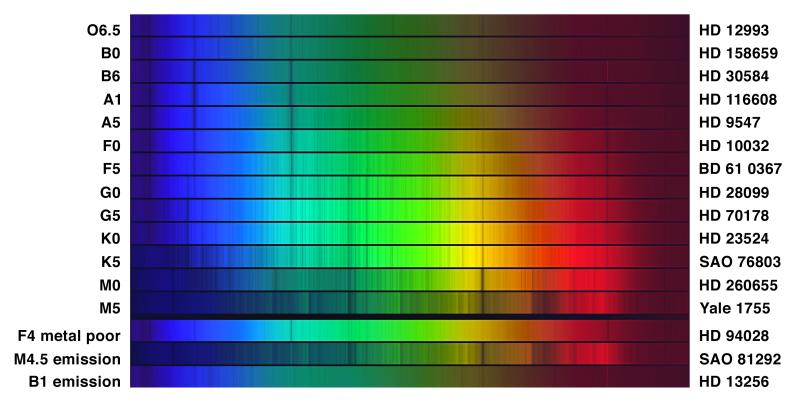
\includegraphics[width=0.95\textwidth]{stellar-spectra.jpg}
\BS

\large

All the stars are made of the same stuff -- the same stuff as we are.\pause
\EC
``The cosmos is also within us. We are made of star-stuff. We are a way for the universe to know itself.''

\begin{flushright}--Carl Sagan, {\it Cosmos} \end{flushright}
}

\frame{\frametitle{\textbf {What a lucky accident!}}
\large 
We're very lucky that atomic transitions happen to lie in our visual range!

There are others that are very interesting to astronomers:

\BI
\item Molecular vibrations: infrared
\pause
\item Molecular {\it rotations}: microwave
\pause
\item ``Hyperfine structure'' energy levels in hydrogen: 21 cm radio waves
\EI

\pause

\normalsize

This last is particularly interesting: it is a very particular frequency, echoing out from
all corners of the Universe, that says: hydrogen is here. (Hydrogen is 75\% of the universe.)
}

\frame{
\BC
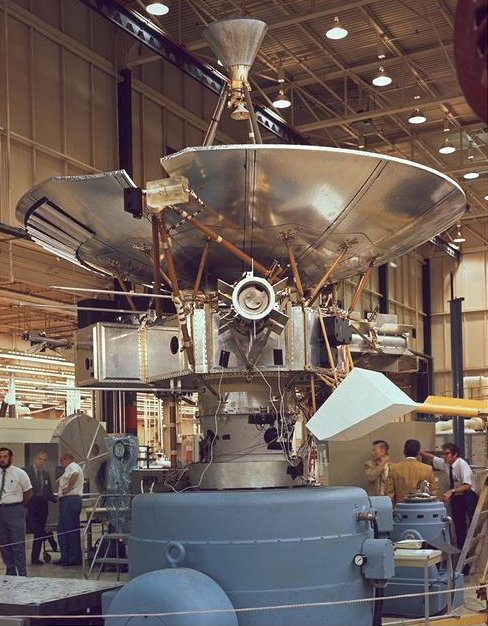
\includegraphics[width=0.5\textwidth]{pioneer-10.jpg}
\EC
}

\frame{
\BC
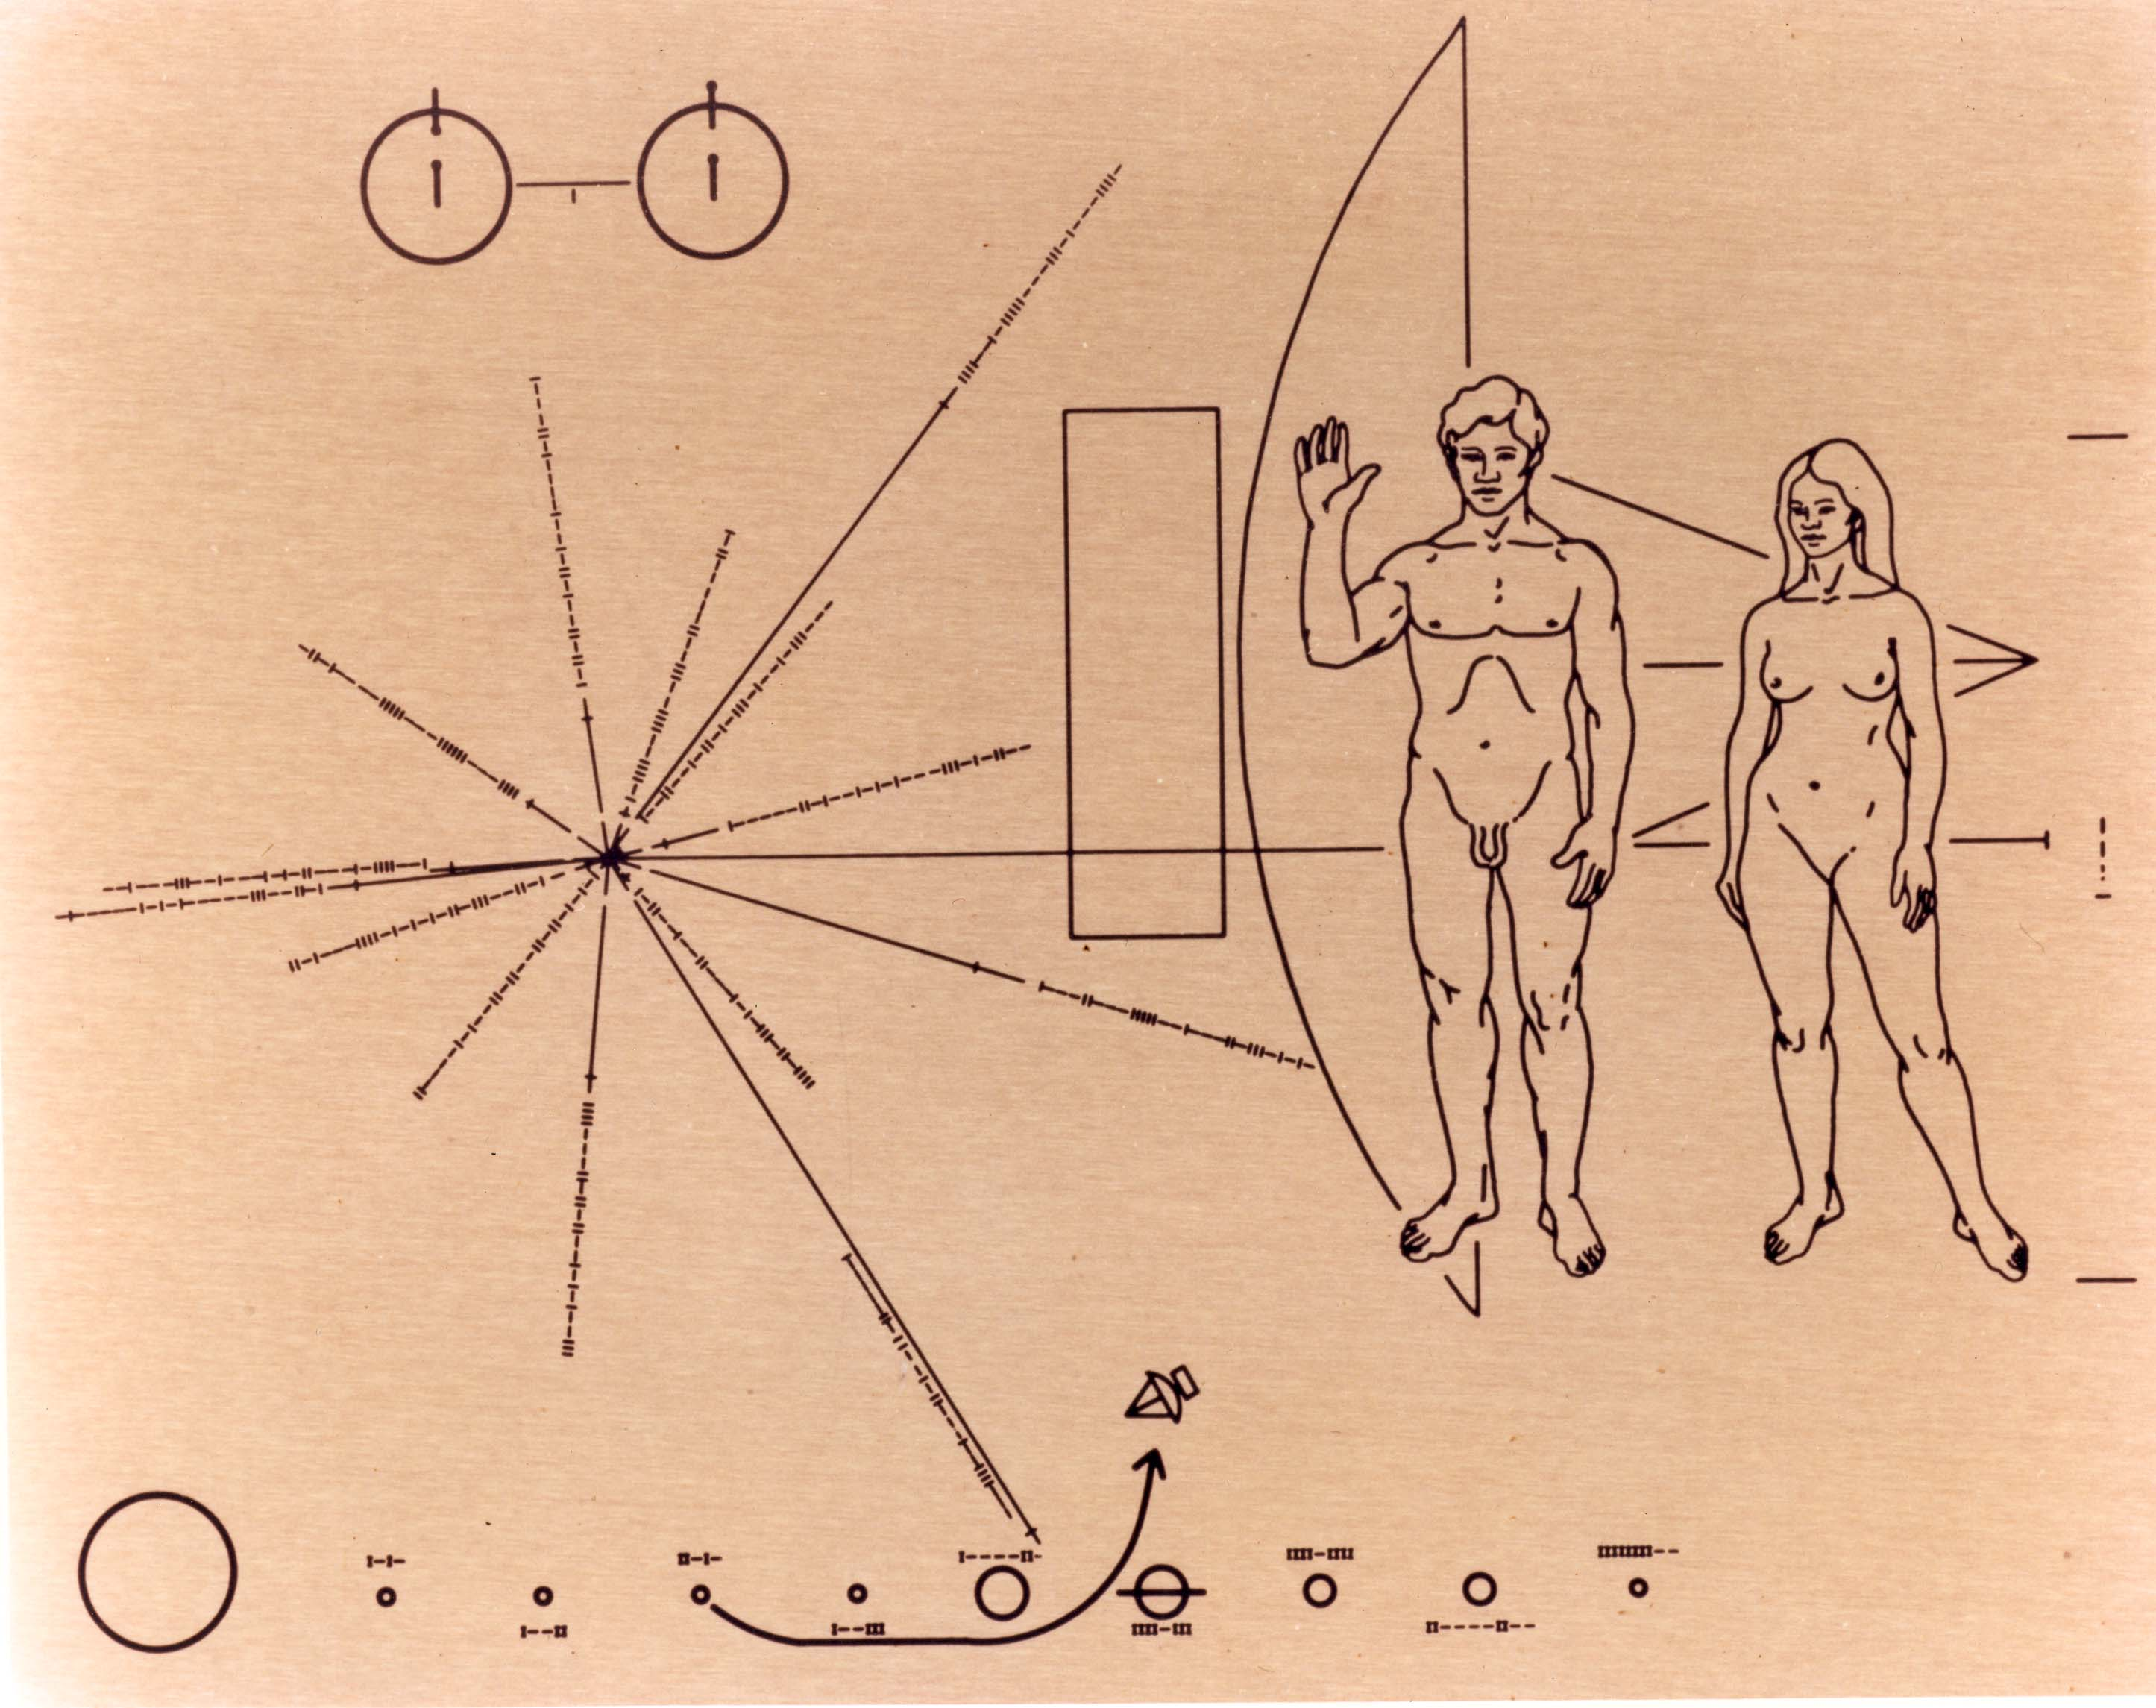
\includegraphics[width=0.8\textwidth]{pioneer-plaque.jpg}
\EC
}

\frame{
\BC
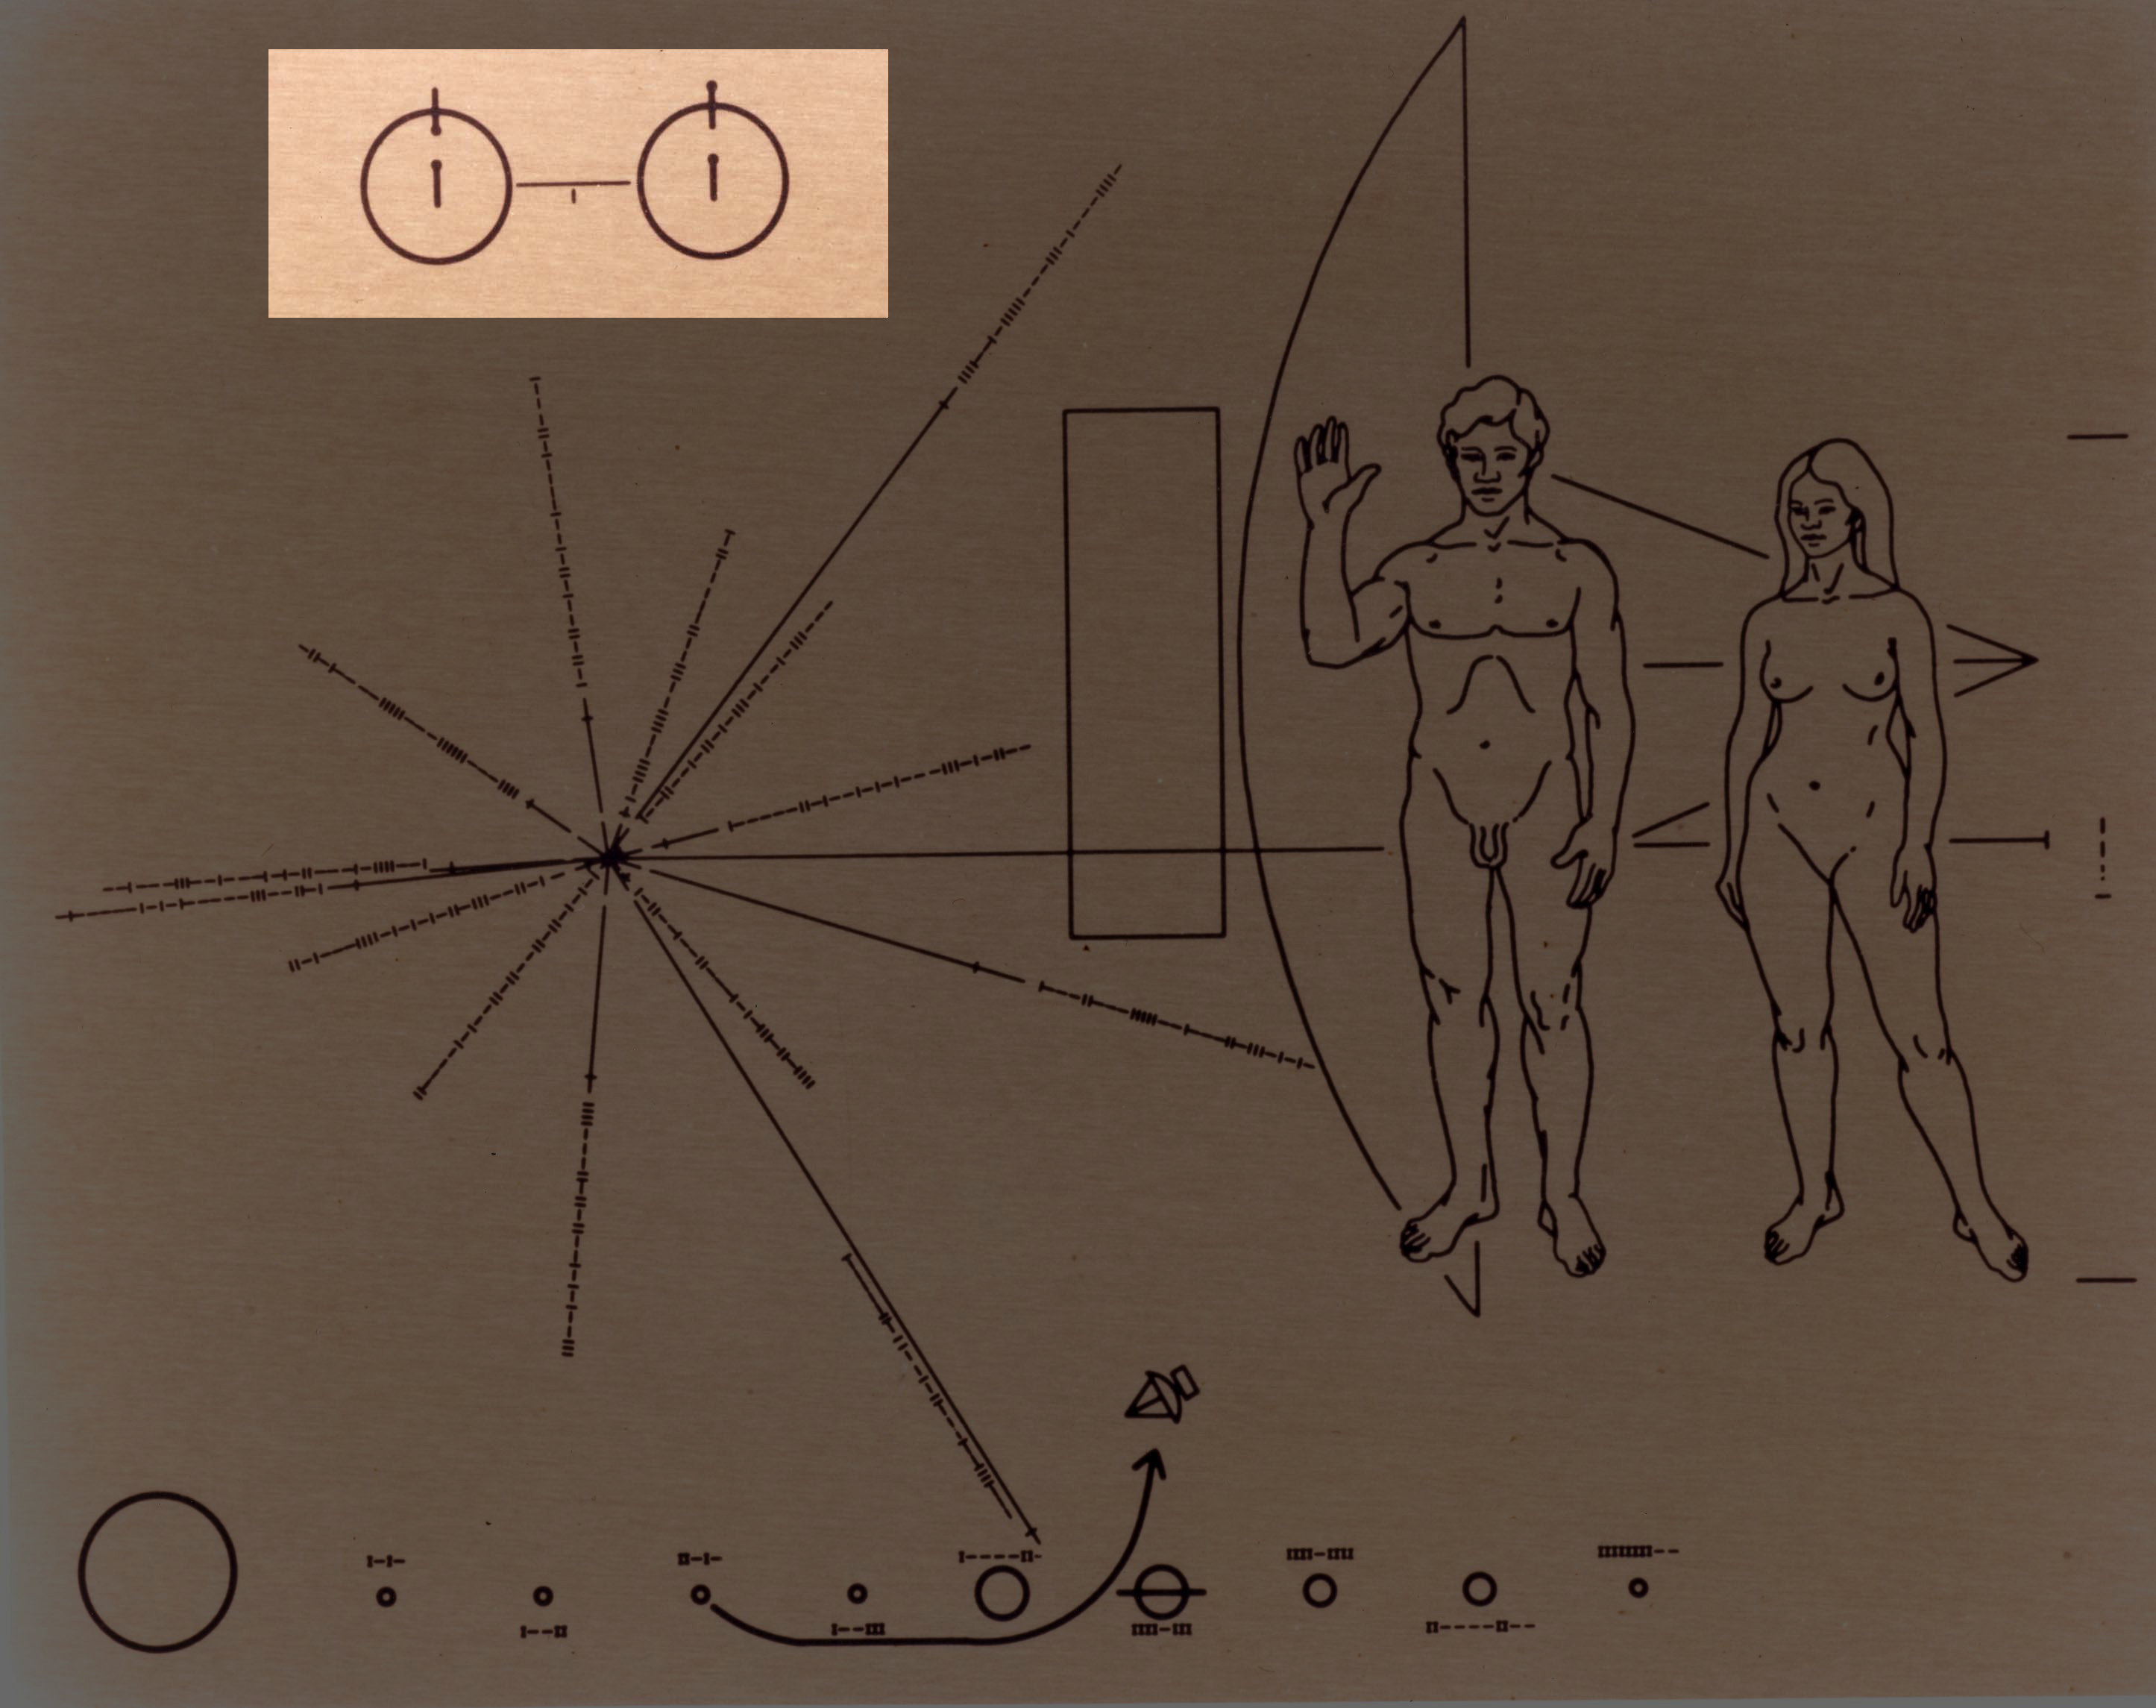
\includegraphics[width=0.7\textwidth]{pioneer-plaque-2.jpg}\\
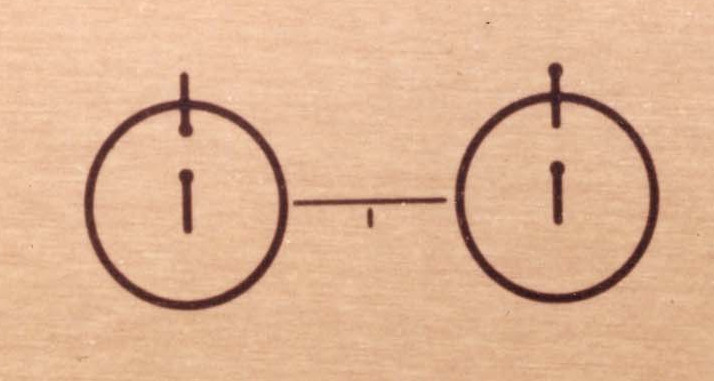
\includegraphics[width=0.3\textwidth]{hyperfine.jpg}
\EC
}

\end{document}

